\begin{figure}[t]
    \centering
    % 第一张图及其标题
    \begin{minipage}[b]{0.32\linewidth}
        \centering
        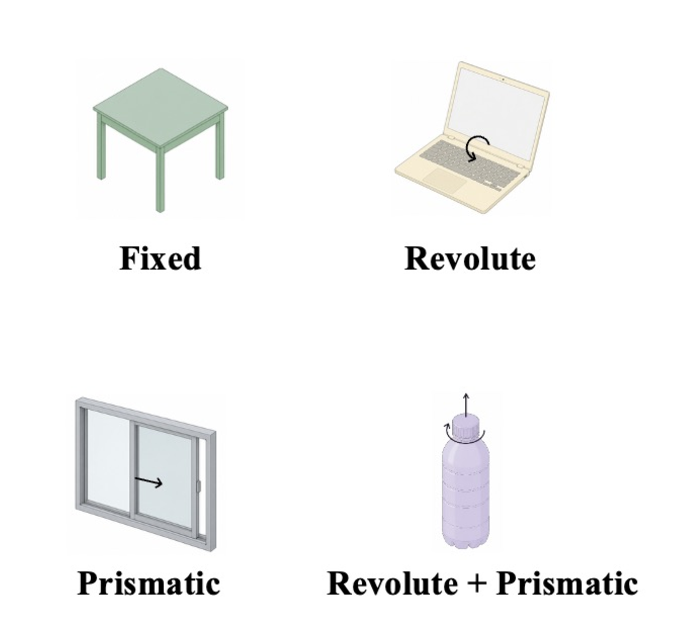
\includegraphics[width=\linewidth]{figs/3_ART_type.pdf}
        \caption{Articulation types.} % 独立的标题 1
        \label{fig:art_type}
    \end{minipage}
    \hfill % 撑开中间间距
    % 第二张图及其标题
    \begin{minipage}[b]{0.65\linewidth}
        \centering
        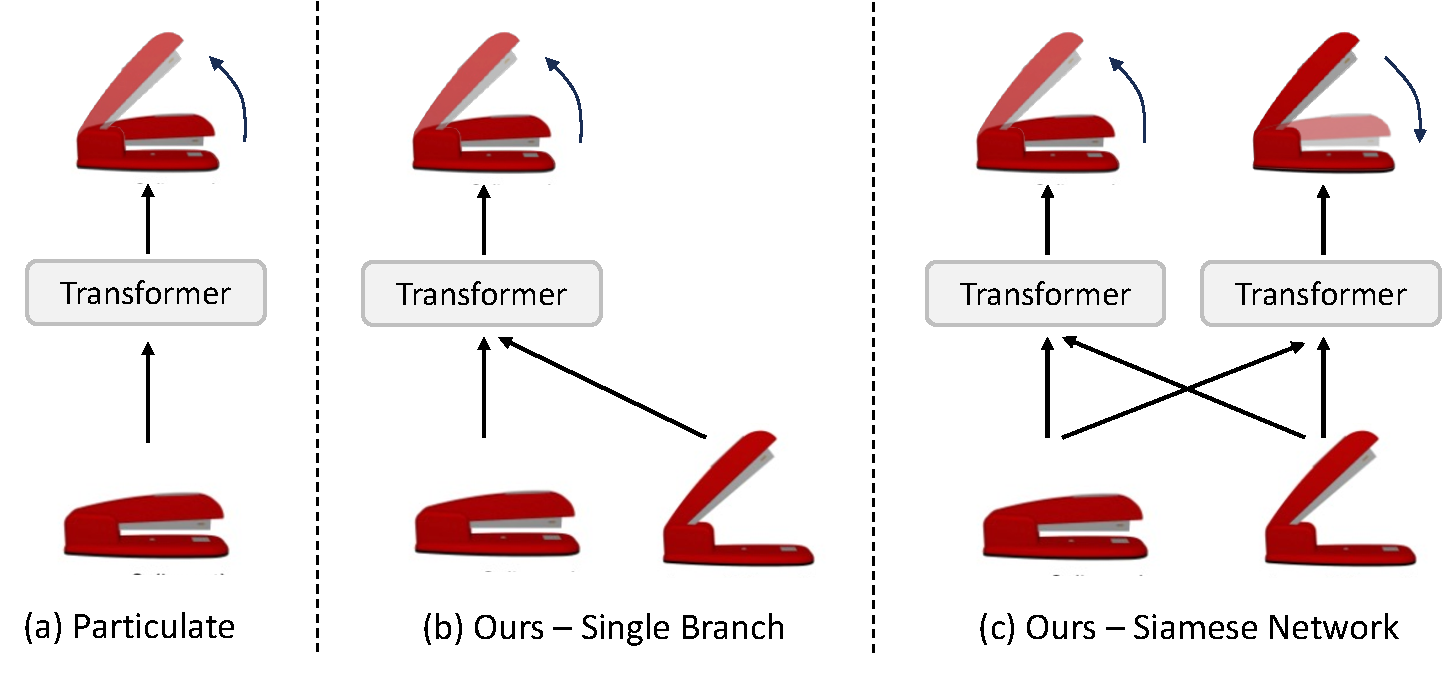
\includegraphics[width=\linewidth]{figs/5_model_diff.pdf}
        \caption{The different pipelines.} % 独立的标题 2
        \label{fig:model_diff}
    \end{minipage}
\end{figure}


\section{Method}%
\label{sec:method}

We introduce \method,
a Siamese transformer architecture for learning part segmentation and articulation parameters from two states ($s_0$ and $s_1$) of an articulated object.
We first formulate the problem setting in~\Cref{sec:problem},
followed by our Siamese transformer architecture in~\Cref{sec:backbone} and its multi-task decoder in~\Cref{sec:decoder}.
Finally, we describe the training objectives in~\Cref{sec:training}.

\begin{figure}[t]
    \centering
    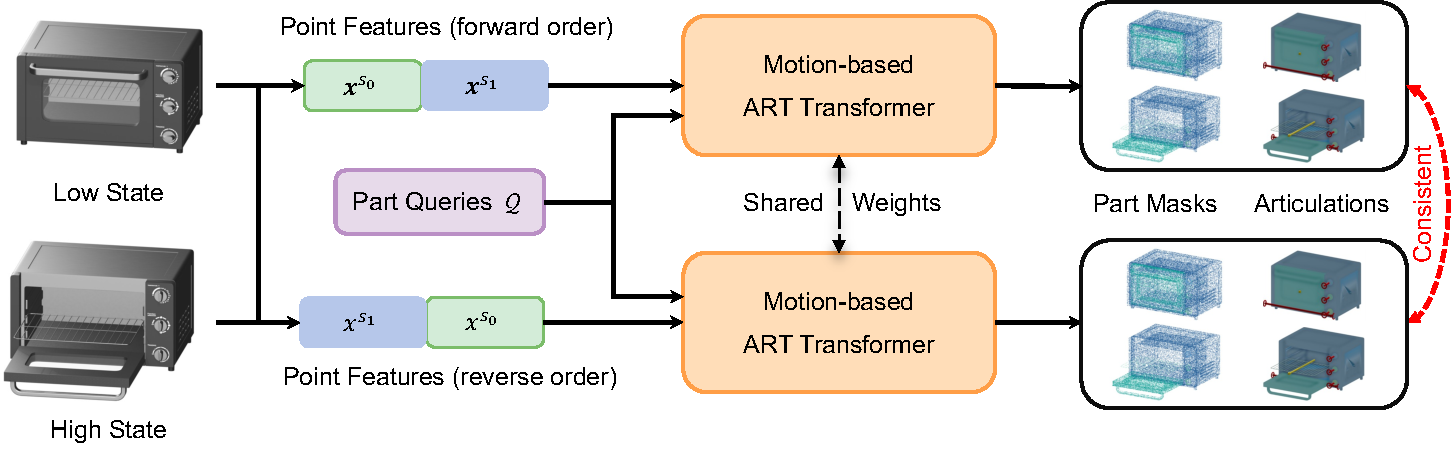
\includegraphics[width=\linewidth]{figs/framework.pdf}
    \caption{\textbf{Overview of \emph{\method}.} Given two observed states of the same object, our framework jointly reasons over cross-state geometry to predict part segmentation and the underlying kinematic structure. We use a set of shared queries to aggregate two-state features, with each query representing a rigid part. The overall Siamese framework consists of two branches: forward order and reverse order. Each branch predicts both part segmentation of two states and articulation parameters.}
    \label{fig:method_overview}
\end{figure}

% \ruijie{
\subsection{Problem Formulation}
\label{sec:problem}
The input is two distinct physical states of an object,
representing the articulation motion from start $s_0$ to end $s_1$.
Specifically, the observations are two unorganized point clouds 
$\{\mathcal{P}^{(s_i)}\}_{i=\{0,1\}}$,
where each
$\mathcal{P}^{(*)} = \{\bm{p}_i^{(*)}\in\mathbb{R}^3\}_{i=1}^N$
is sampled from two states of the object mesh
$\{\mathcal{M}^{(s_i)}\}_{i=\{0,1\}}$,
respectively,
where $N$ is the number of sampled points.
Our goal is to learn a Model
$f_{\bm{\theta}}$
that maps these two states of point clouds to a set of part segmentation masks and articulation parameters:
\begin{equation}
    \label{eq:goal}
    f_{\bm{\theta}} : \{\mathcal{P}^{(s_i)}, \mathcal{N}^{(s_i)}, \bm{F}^{(s_i)}\}_{i=\{0,1\}} \mapsto \{M^{(s_i)}, \mathcal{G}^{(s_i)}, \Theta^{(s_i)}\}_{i=\{0,1\}},
\end{equation}
where $\mathcal{N}^{(s_i)}$ and $\bm{F}^{(s_i)}$ are the surface normal and part features from off-the-shelf extractors of the point cloud from state $s_i$, respectively.

We predict all outputs for both states.
However, to simplify the notation, we will only describe the output of one state, while the other state follows the same procedure.
We predict the segmentation masks $M \in \{0,1\}^{N \times K}$ for $K$ \emph{kinematic parts}
and infer the underlying \emph{kinematic graph}
$\mathcal{G} = \{\mathcal{V}, \mathcal{E}\}$,
where
node $\mathcal{V}$ composed by $K$ kinematic parts and
edge $\mathcal{E}$ is a directed \emph{kinematic tree}
$J_{K \times K}$
that defines the joint connectivity between parts.
We also predict the \emph{articulation parameters} of joints $\Theta=\{\mathcal{A}, \mathcal{R}, \mathcal{T}\}$,
where
$\mathcal{A}$ denotes the articulation types,
which are predefined as four types:
$\{$fixed, \emph{revolute}, \emph{prismatic}, and \emph{revolute + prismatic}$\}$, as shown in~\Cref{fig:art_type};
$\mathcal{R} = \{(\bm{\omega}_e, \bm{q}_e, \alpha_e)\}_{e \in \mathcal{E}}$ denotes the revolute parameters, where $\bm{\omega}_e \in \mathbb{S}^2$ is a unit rotation-axis direction, $\bm{q}_e \in \mathbb{R}^3$ is a pivot point on that axis, and $\alpha_e \in \mathbb{R}$ is the range
$(\alpha_{\min}, \alpha_{\max})$
of the rotation angle between two states;
and $\mathcal{T} = \{(\bm{d}_e, l_e)\}_{e \in \mathcal{E}}$ denotes the prismatic parameters,
where $\bm{d}_e \in \mathbb{S}^2$ is a unit translation direction and $l_e \in \mathbb{R}$ is the range
$(l_{\min}, l_{\max})$
of the translation distance between two states.

\heading{\emph{Multi}-state \vs \emph{single}-state}
We implement the model
$f_{\bm{\theta}}$
as a feed-forward Siamese transformer architecture
with shared weights,
and $\bm{\theta}$ are the learnable parameters.
Prior feed-forward methods~\cite{chen2024urdformer,chen2025ArtiLatent,che2024op,Goyal_2025_ICCV,li2025particulate} usually optimize $\bm{\theta}$ with a single state as input.
This is partly reliable if the training data is sufficiently large and diverse in the deep learning era, but it is \emph{not} the case in practice, especially for kinematic annotated 3D.
We instead consider a new \emph{feed-forward} paradigm that uses \emph{two-state} of an object as input to learn the underlying physical rules of articulation from the state motion change,
which is more efficient and generalizable than learning priors from a single state.
The \emph{core insight} is that the two states of the same object directly reveal the articulation attributes,
while two-state observations are also easily obtained in real-world applications, \eg, by scanning or capturing an object before and after interaction.
Notably, we do \emph{not} assume any point correspondence between two states,
which is more challenging but also more practical in real-world applications.
We select \emph{two}-state because it is the minimum number of states that can reveal the articulation attributes,
but our design is \emph{not} specific to two states and can be easily extended to more states if needed.

% \subsection{Overall Framework}
% As shown in~\Cref{fig:method_overview}, our method, \method, addresses this problem with a Siamese transformer framework. 
% First, we extract features from two point clouds, $P_0$ and $P_1$, and concatenate the resulting feature sets to serve as context information, in ascending and descending order, respectively. 
% A set of part queries is then initialized to perform cross-attention on the context features in each branch.
% The updated part queries are finally passed through the ART Decoder to predict the part segmentation and articulation parameters.
% We use ground-truth annotations for segmentation and articulation supervision and design a consistency loss to further enforce symmetry between the two dual branches.
% The overall framework offers two-sided advantages:
% (1) efficient learning, since the Siamese network is trained on two dual samples in each iteration;
% (2) fast inference speed, since we only need a single branch for inference.
% }
% The two states are processed as separate point streams, but they are interpreted by a single set of part queries that is reused across both states. 
% This design ensures that each query represents the same semantic and kinematic part before and after motion, thereby avoiding the need to solve an additional query-matching problem across states. 
% The resulting part queries are used by a Mask2Former-style mask refinement decoder and by kinematic heads that predict part connectivity, motion type, and joint parameters.

\subsection{Two-state Motion-based Articulation Transformer}
\label{sec:backbone}

At a high level, \method is a Siamese transformer architecture with shared weights that takes two states of point clouds as input,
and learn the underlying physical rules of articulation from the state motion change,
rather than learning articulation priors from a single state as in prior feed-forward methods~\cite{li2025particulate,li2025urdfanything,wu2026urdfanything_plus}.
The key insight of our design is that we can simultaneously infer full articulation attributes for two states,
using only one set of shared part queries,
and achieve more robust, generalizable performance by enforcing cycle consistency between them.

However, this architecture design is non-trivial because: 
(1) The two states of point clouds are randomly sampled and unorganized, \ie, there are no matching points between the two states. 
\footnote{Note that we deliberately did not perform consistent sampling of the point clouds to generate data samples, because it is too difficult to obtain the matching points in the second state as input in practical applications.}
(2) The motion of articulated parts makes the point correspondence more complex, \ie, those points of the moving parts are not even spatially aligned.
The missing point correspondence indicates that although the additional state provides richer articulation cues, the network still requires careful design to fully utilize them.
To address this issue, we develop a dedicated two-state Motion-based Articulation Transformer with a Siamese architecture.

\heading{Siamese Architecture with Shared Part Queries}
As shown in~\Cref{fig:model_diff} (a),
prior feed-forward methods predict full articulation parameters by learning from a single state of an object.
However, our model includes two states of an object as input.
We could instead train the network by directly concatenating the two states with $2N$ points
as input and predicting the full articulation attributes for both states at the same time (\Cref{fig:model_diff} (b)). 
While this na\"ively concatenation works by learning with two states,
it does not explicitly enforce the part queries to learn the same semantic and kinematic part across two states.
More importantly,
since we argue the \emph{two-state} learning paradigm learns articulation in a way that aligns with physical laws, as it captures the underlying motion between two states rather than the instance category.
Hence, if we swap the order of the observed states, the model should still produce correct and consistent predictions.
We achieve this by designing a Siamese architecture with shared weights and part queries (\Cref{fig:model_diff} (c)).
Enforcing consistency between two branches using the cycle consistency loss yields more robust and generalizable performance, as shown in our experiments.
% \heading{Masked Query-to-point Attention} \cxz{remove it as it does not mean a lot from the ablations}
Our transformer architecture is inspired by Particulate~\cite{li2025particulate},
but features several key differences that allow us to train with two states and ensure the consistency between the two branches.

For each \textbf{input} point
$\bm{p}_i\in\mathcal{P}$,
we still concatenate its coordinates, normals, and part features in the channel dimension to obtain the input point features
$\bm{x}_i = \big[\,\bm{p}_i, \bm{n}_i, \bm{f}_i\,\big] \in \mathbb{R}^{3 + 3 + d}$.
But now we have two states of points that are concatenated in the token dimension, \ie, $\{\bm{x}_i\}_{i=1}^{2N}$.
In our final reverse-order modal (\Cref{fig:method_overview} (c)),
we simply swap the order of two states of input point features.

For the \textbf{part queries},
we still use a set of shared learnable queries $\mathcal{Q} \in \mathbb{R}^{K_{\max} \times D}$,
where $K_{\max}$ is set to be particularly large to cover the maximum number of parts in the training data,
as the actual number of parts is unknown a priori,
and $D$ is the query dimension.

The \textbf{attention blocks} 
is a sequence of self-attention on part queries, followed by query-to-point attention and point-to-query attention.
Here, we apply the masked attention mechanism~\cite{cheng2022masked} to the query-to-point attention,
which first predicts a binary mask for each query to indicate the activated points,
and then uses the predicted mask to modulate the attention weights in the next layer of attention.
The detailed description is provided in~\Cref{sec:supp_impl_compute_impact}.
This masked attention mechanism is crucial for our model to learn from two states without point correspondence,
as it forces the part queries to focus on the activated areas of the same part across two states.
After several layers of attention, we obtain the updated part queries
$\tilde{\mathcal{Q}} \in \mathbb{R}^{K_{\max} \times D}$,
and point tokens $\tilde{\mathcal{P}} \in \mathbb{R}^{2N \times D}$.

\subsection{Prediction Heads}
\label{sec:decoder}
Following Particulate~\cite{li2025particulate}, we use several MLPs to predict the part segmentation
$M$,
the kinematic graph $\mathcal{G}$,
and the articulation parameters $\Theta$.
Note that we primarily describe the decoding process for the forward-order branch, while the other branch follows a similar procedure.

We use an MLP to predict the \textbf{point segmentation mask}
$\hat{M} = \operatorname{MLP} (\tilde{\mathcal{Q}}, \tilde{\mathcal{P}})$,
where $\hat{M}\in \mathbb{R}^{2N \times K_{\max}}$,
which indicates the probability of part segmentation for each point.
Note that it contains points from both states,
even in one branch.

We predict the \textbf{kinematic graph} $\hat{\mathcal{G}}$,
which is represented as a kinematic tree $\hat{J} \in \{0,1\}^{K_{\max} \times K_{\max}}$,
by applying an MLP to every ordered query pair
$\hat{J}_{ij} = \operatorname{MLP} (\tilde{Q}_i,\tilde{Q}_j)$,
where $\tilde{Q}_i,\tilde{Q}_j$ correspond to the corresponding query of part $i$ and $j$, respectively.
Following the URDF definition, we designate one basic part as the root node of the kinematic tree and restrict each part to have at most one parent node.
Therefore, given actual $K$ parts, there are exactly $K-1$ joints,
where $K \le K_{\max}$.

We use several MLPs to predict the \textbf{articulation parameters} $\hat{\Theta} =\operatorname{MLPs} (\tilde{\mathcal{Q}})$,
where $\hat{\Theta} = \{\hat{\mathcal{A}}, \hat{\mathcal{R}}, \hat{\mathcal{T}}\}$.
Note that,
separate MLPs are used to predict different types of parameters in $\hat{\Theta}$.
As mentioned in~\Cref{sec:problem},
we predefine four types of articulation.
The articulation type $\hat{\mathcal{A}}$ is predicted by a classification MLP to output the logits of query part $i$ belonging to each of the \emph{four} types.
The revolute parameters $\hat{\mathcal{R}} = \{\hat{\bm{\omega}}_e, \hat{\bm{q}}_e, \hat{\alpha}_e\}_{e\in\mathcal{E}}$
and prismatic parameters $\hat{\mathcal{T}} = \{\hat{\bm{d}}_e, \hat{\bm{q}}_e\}_{e\in\mathcal{E}}$ are predicted by regression MLPs for each joint $e$.
Note that the predicted parameters of a joint are only valid if the corresponding part is classified as a moving part, \ie, revolute, prismatic, or revolute + prismatic.

% Our predication heads are mainly built on Particulate~\cite{li2025particulate},
% which is not our main contribution.
% For more details of the architecture design and implementation, please refer to~\cite{li2025particulate}.

\subsection{Training}
\label{sec:training}

During training, we sample two point cloud states and their corresponding ground-truth annotations.
Note that,
while we have different states,
the kinematic tree, articulation type, and joint parameters should be the same for both states.
We only swap the part segmentation masks between the two states, and also flip the ranges of revolute and prismatic motion to align the motion directions.
This design enforces the model to learn the same kinematic structure and motion attributes across two states.

% We train \method end-to-end. For each training sample, we extract its two-state point cloud as input and have the siamese network predict, for each branch, the part segmentation $M$, the kinematic tree $J$, and the articulation parameters $\theta = \{A, R, T\}$.
% Meanwhile, the corresponding ground truth annotations are curated to provide direct supervision.
% However, the predicted class-agnostic parts do not correspond to the ground truth on a one-to-one basis; we still need a matching procedure for backpropagation. 

\heading{Part Matching with Ground Truth}
We use the Hungarian Matching to build part correspondence following~\cite{li2025particulate,carion2020end}. The difference with~\cite{li2025particulate} is that since we have two sets of output queries that predict two-state part segmentation, we only perform Hungarian Matching for the rest state and enforce the articulated state following the same matching orders. 
In this way, we ensure that the two output queries predict consistent part segmentation.

\heading{Training Losses}
We train the \method end-to-end using a multi-task loss:
\begin{equation}
    \label{eq:total_loss}
    \mathcal{L} = \underbrace{\mathcal{L}_\text{seg}^\text{f}+\mathcal{L}_\text{art}^\text{f}}_\text{forward branch loss} + \underbrace{\mathcal{L}_\text{seg}^\text{r}+\mathcal{L}_\text{art}^\text{r}}_\text{reverse branch loss} +  \underbrace{\lambda_\text{cycle} \mathcal{L}_\text{cycle}}_\text{cycle loss},
\end{equation}
where $\mathcal{L}^{*}_\text{seg}=\sum_{i=\{0,1\}}\operatorname{CE}(\hat{M}^{(s_i)}, M^{(s_i)})$ is the cross entropy loss for \textbf{part segmentation} for both states
$s_i$ in branch $*$,
$\mathcal{L}^{*}_\text{art} = \operatorname{BCE}(\hat{\mathcal{J}},\mathcal{J}) + \operatorname{CE}(\hat{\mathcal{A}},\mathcal{A}) + \ell_1(\hat{\mathcal{R}}, \mathcal{R}) + \ell_1(\hat{\mathcal{T}}, \mathcal{T})$
is the \textbf{articulation loss} for branch $*$,
which includes binary cross-entropy loss for the kinematic tree $\mathcal{J}$, cross-entropy loss for the articulation type $\mathcal{A}$, and L1 losses for the revolute parameters $\mathcal{R}$ and prismatic parameters $\mathcal{T}$.
The motion ranges of revolute and prismatic joints in the two branches are flipped.
To simplify the notation,
we just use $\mathcal{R}$ and $\mathcal{T}$ to represent them.
More details are provided in~\Cref{sec:supp_loss_details}.

Since the two branches solve dual problems,
we can naturally construct \textbf{cycle consistency loss}
$\mathcal{L}_{cycle}$ between the branches,
which includes both the part segmentation loss and the articulation loss:
\begin{equation}
    \mathcal{L}_\text{cycle} =
    \operatorname{BCE}(\hat{\mathcal{J}_f},\hat{\mathcal{J}_r}) + \operatorname{CE}(\hat{\mathcal{A}_f},\hat{\mathcal{A}_r}) + \ell_1(\hat{\mathcal{R}_f},\hat{\mathcal{R}_r}) + \ell_1(\hat{\mathcal{T}_f},\hat{\mathcal{T}_r})
    + \sum_{i=\{0,1\}}\operatorname{CE}(\hat{M}^{(s_i)}_f, \hat{M}^{(s_i)}_r)
\end{equation}
where the lower script $f$ and $r$ denote the forward-order branch and reverse-order branch, respectively.
This cycle consistency loss enforces that the two branches produce consistent predictions, leading to more robust and generalizable performance, as shown in our experiments.

% \hrule

% \ruijie{

% \paragraph{Cycle Consistency loss.}
% Since the two branches solve dual problems, we can naturally construct consistency constraints between the branches. Specifically, for the reverse-order branch, we swap the part segmentation predictions to match the parts and flip the ranges of revolute and prismatic motion to align the motion directions. The cycle consistency loss includes both the part segmentation loss and the articulation loss:
% \begin{equation}
%     \mathcal{L}_{cycle} = \sum_{i=\{0,1\}}\text{CE}(M_i, \widetilde{M}_{1-i}) + \sum \left ( \text{BCE}(J,\widetilde{J}) + \text{CE}(A,\widetilde{A}) + ||R+\widetilde{R}||_1 + ||T+\widetilde{T}||_1\right )
% \end{equation}
% where $\widetilde{M},\widetilde{J},\widetilde{A},\widetilde{R},\widetilde{T}$ are the prediction results of the reserve-order branch.
% }

% \paragraph{Total loss.}
% The final training loss is summarized as:
% \begin{equation}
%     \mathcal{L}_{total} = \underbrace{\mathcal{L}_{seg\_1}+\mathcal{L}_{art\_1}}_{branch~1~loss} + \underbrace{\mathcal{L}_{seg\_2}+\mathcal{L}_{art\_2}}_{branch~2~loss} +  \underbrace{\lambda_{cycle} \mathcal{L}_{cycle}}_{cycle~loss}
% \end{equation}
% }

% \method is trained with supervision on segmentation, kinematic structure, motion class, and continuous motion parameters. The segmentation objective combines pointwise cross-entropy and Dice loss over the concatenated two-state masks. The graph decoder is trained with binary cross-entropy over valid part pairs, and the motion classifier is trained with cross-entropy over valid parts. Continuous joint parameters are supervised with L1 losses on active revolute and prismatic joints, while inactive motion heads are ignored through valid-motion masks. For the closest-axis representation, we additionally supervise the predicted closest point on the revolute axis for points belonging to revolute parts. The final objective is a weighted sum of these terms:
% \begin{equation}
%     \mathcal{L} =
%     \lambda_{\mathrm{mask}}\mathcal{L}_{\mathrm{ce}} +
%     \lambda_{\mathrm{dice}}\mathcal{L}_{\mathrm{dice}} +
%     \lambda_{\mathrm{edge}}\mathcal{L}_{\mathrm{edge}} +
%     \lambda_{\mathrm{cls}}\mathcal{L}_{\mathrm{motion}} +
%     \lambda_{\mathrm{param}}\mathcal{L}_{\mathrm{param}} +
%     \lambda_{\mathrm{axis}}\mathcal{L}_{\mathrm{closest}}.
% \end{equation}
% This objective encourages the shared part queries to explain both observed states consistently while still preserving point-level evidence for precise mask and joint prediction.

